\section{業務の流れ}
% ここから本文を書いてください.
本システムは、主に授業中の質問や進捗状況をリアルタイムで表示することで、授業の支援を行うシステムです。

管理者は、本システムが内蔵されているRaspberry Pi 3を、管理者用のPCに接続することで利用可能になります。
管理者が担当してある授業に合わせて進捗状況の可視化や、質問の蓄積についてを設定できます。
学生側は、このRaspberry Pi 3にWi-Fiで接続することで、本システムが利用可能になります。

本システムでは、進捗状況を管理側の画面で確認できるため、与えられた課題に対して、各学生の進み具合を把握することができます。
各学生は、質問をスマートフォンなどの端末から送信することができ、この質問は管理者用の画面に表示されます。
管理者は、画面上でこの質問に回答することができます。
また、これらの質問や回答は、Raspberry Pi 3のデータベースに蓄積されます。
このデータは管理者や学生が確認できるため、過去の質問を参考に現在の授業に取り組むことも可能となっています。

\begin{figure}[htbp]
  \begin{center}
    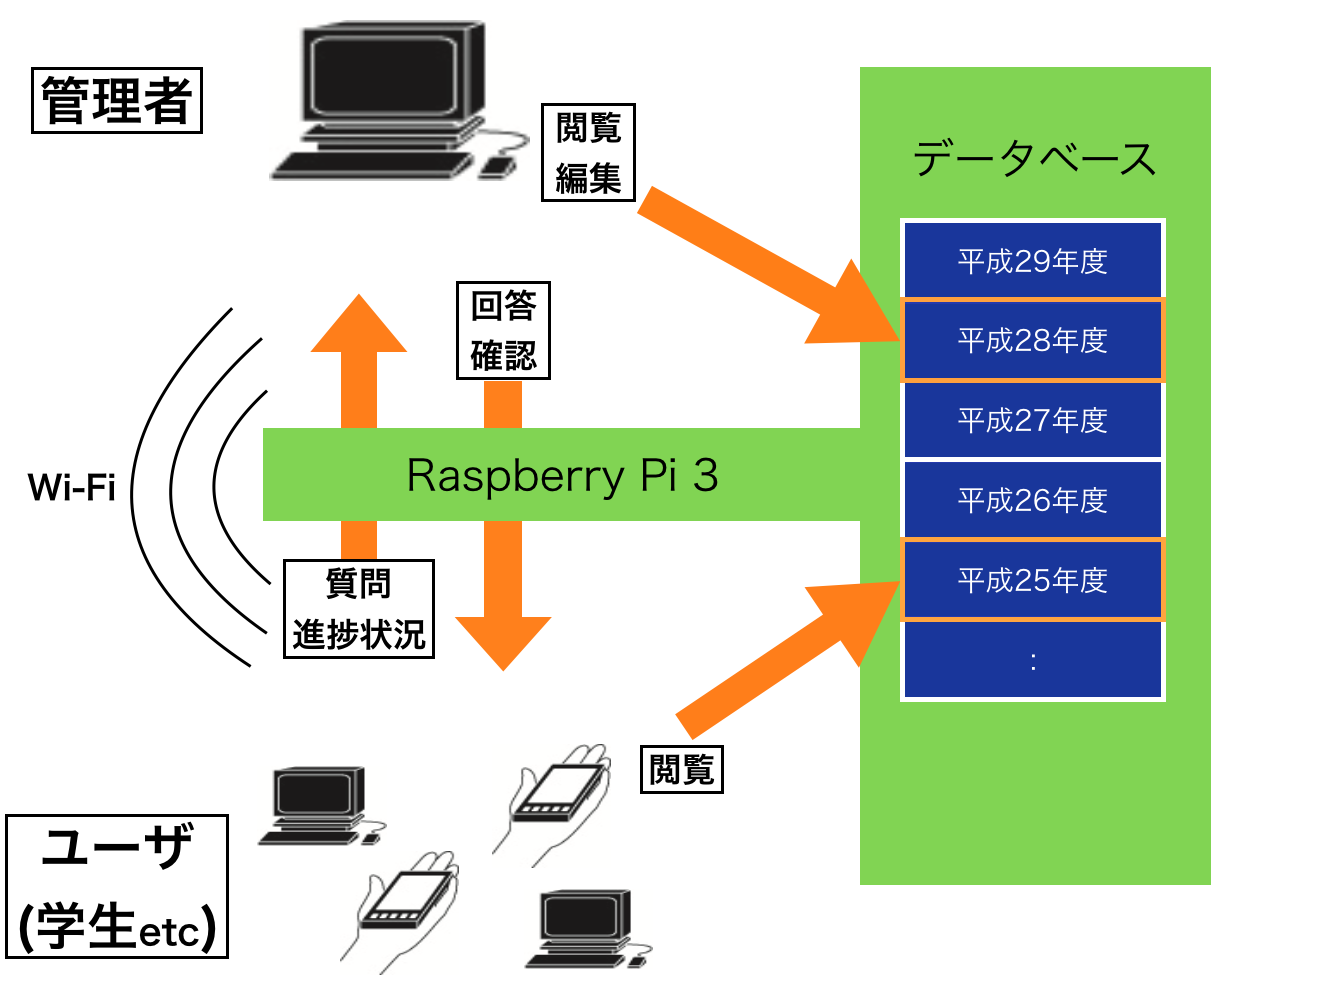
\includegraphics[width=1\linewidth,clip]{./img/flow.png}
    \caption{業務の流れ}\label{fig:flow}
  \end{center}
\end{figure}
